% =====================================================================
%  Revised paper template (BEEI-like layout)
%  If you have the official BEEI class/template, copy the body sections
%  (from \section{Introduction} onward) into it instead.
%  Figures are expected in ./plots_final/ (output of plot_results.py)
% =====================================================================
\documentclass[10pt,a4paper]{article}

\usepackage[margin=2cm]{geometry}
\usepackage{amsmath,amssymb}
\usepackage{graphicx}
\usepackage{booktabs}
\usepackage{multirow}
\usepackage{caption}
\usepackage{subcaption}
\usepackage{enumitem}
\usepackage{xcolor}
\usepackage[hidelinks]{hyperref}
\usepackage{titlesec}
\usepackage{fancyhdr}

% --- BEEI-like headings: "1. INTRODUCTION", "2.1. Subsection" ---
\titleformat{\section}{\normalfont\bfseries}{\thesection.}{1em}{\MakeUppercase}
\titleformat{\subsection}{\normalfont\bfseries}{\thesubsection.}{0.6em}{}
\renewcommand{\thesubsection}{\thesection.\arabic{subsection}}

\pagestyle{fancy}
\fancyhf{}
\fancyhead[L]{\small Bulletin of Electr Eng \& Inf}
\fancyhead[R]{\small ISSN: 2302-9285}
\fancyfoot[C]{\small \thepage}

% Placeholder helper — search for \todo to find everything left to write
\newcommand{\todo}[1]{\textcolor{red}{[TODO: #1]}}

\title{\bfseries Reinforcement Learning with an AI Director for\\ Dynamic Difficulty Adjustment in Survival Games}
\author{
Kabengele Bwateketa\textsuperscript{1}, Michael Anokye-Boateng\textsuperscript{2}, Oluwarotimi Randle\textsuperscript{3}\\[4pt]
\small \textsuperscript{1,2}School of Computer Science \& Applied Mathematics, University of the Witwatersrand, Johannesburg, South Africa\\
\small \textsuperscript{3}Digital Arts, University of the Witwatersrand, Johannesburg, South Africa
}
\date{}

\begin{document}
\maketitle

% ---------------------------------------------------------------------
\noindent
\begin{minipage}[t]{0.28\textwidth}
\small
\textbf{Article Info}\\[4pt]
\textit{Article history:}\\
Received month dd, yyyy\\
Revised month dd, yyyy\\
Accepted month dd, yyyy\\[6pt]
\textit{Keywords:}\\
Dynamic Difficulty Adjustment\\
Reinforcement Learning\\
Q-learning\\
AI Director\\
Player Modelling
\end{minipage}\hfill
\begin{minipage}[t]{0.68\textwidth}
\small
\textbf{ABSTRACT}\\[4pt]
\todo{Context (1--2 sentences). Method: tabular Q-learning agent, Unity survival game,
four conditions (Easy, Baseline, Hard, AI Director), 3 seeds $\times$ 600 episodes,
random-policy baselines and greedy evaluation. Key results with numbers. One-sentence,
appropriately scoped conclusion.}
\end{minipage}

\vspace{6pt}
\noindent\small\textit{This is an open access article under the CC BY-SA license.}
\normalsize

\vspace{6pt}
\noindent\textbf{Corresponding Author:}\\
\todo{Name, affiliation, email}

% =====================================================================
\section{Introduction}
\todo{Motivation for DDA and AI Directors in games.}

\todo{Gap: how adaptive difficulty affects the learning of an RL agent (not human players).}

\todo{Contributions / research questions --- keep claims scoped to what was measured.}
\begin{enumerate}[label=(\roman*)]
    \item \todo{Contribution 1}
    \item \todo{Contribution 2}
\end{enumerate}

% =====================================================================
\section{Related Work}
\todo{DDA background [Hunicke 2005], AI Directors, RL-based DDA, player modelling.}

% =====================================================================
\section{Methods}

\subsection{Research design}
\todo{Controlled simulation experiment; four difficulty conditions; what changed since the
previous version (seeding, random baselines, evaluation, reward scaling removed).}

\subsection{Game environment}
\todo{Unity arena, zombies (detection/alerting, wander, chase, attack recovery),
pickups (need-weighted spawning), invulnerability and knockback, 120\,s episode timeout
= win condition.}

\subsection{State and action space}
The state is represented by four discretised variables
(Table~\ref{tab:state}), giving $3^4 = 81$ states.

\begin{table}[h]
\centering
\caption{State variables}
\label{tab:state}
\begin{tabular}{lll}
\toprule
Variable & Categories & Definition \\
\midrule
Enemy proximity (alerted) & near / medium / far & \todo{thresholds} \\
Ammunition & empty / low / ok & \todo{thresholds} \\
Health & critical / hurt / ok & \todo{thresholds} \\
Pickup distance & none / near / far & \todo{thresholds} \\
\bottomrule
\end{tabular}
\end{table}

\noindent Actions (with availability masking):
\begin{itemize}
    \item \textbf{Hold position} --- always available.
    \item \textbf{Flee} --- \todo{availability condition}
    \item \textbf{Move to pickup} --- \todo{}
    \item \textbf{Shoot} --- \todo{}
    \item \textbf{Dash} --- \todo{}
\end{itemize}

\subsection{Tabular Q-learning agent}
\begin{equation}
Q(s,a) \leftarrow (1-\alpha)\,Q(s,a) + \alpha\left[r + \gamma \max_{a' \in \mathcal{A}(s')} Q(s',a')\right]
\end{equation}
\todo{Optimistic initialisation, action masking, terminal vs timeout bootstrapping,
$\varepsilon$-greedy with exponential decay (cite Sutton \& Barto 2018; Singh et al.\ 2000).}

\begin{table}[h]
\centering
\caption{Training parameters}
\label{tab:params}
\begin{tabular}{ll}
\toprule
Parameter & Value \\
\midrule
Episodes per run & 600 \\
Seeds & 42, 43, 44 \\
Learning rate $\alpha$ & 0.1 (constant) \\
Discount factor $\gamma$ & 0.95 \\
Exploration $\varepsilon$ & $1.0 \rightarrow 0.02$, decay 0.985/episode \\
Q-value initialisation & 1.0 \\
Decision period & 0.5\,s \\
Episode timeout & 120\,s \\
Evaluation & 50 greedy episodes per seed ($\varepsilon=0$) \\
Random baseline & 100 episodes per condition \\
\bottomrule
\end{tabular}
\end{table}

\subsection{Reward function}
\todo{Survival reward per decision, kill reward, health-loss penalty, pickup rewards,
death penalty. State that reward is identical across all conditions (no scaling).}

\begin{table}[h]
\centering
\caption{Reward components}
\label{tab:reward}
\begin{tabular}{ll}
\toprule
Event & Reward \\
\midrule
Survival (per decision) & +0.1 \\
Zombie killed & +0.5 \\
Health pickup & +0.3 \\
Ammo pickup & +0.3 \\
Health loss & $-0.05 \times$ damage fraction \todo{check} \\
Death & $-10$ \\
\bottomrule
\end{tabular}
\end{table}

\subsection{Player model and AI Director}
\begin{equation}
T = 0.7\,\text{Stress} + 0.1\,\text{Fatigue} + 0.2\,\text{Engagement}
\end{equation}
\todo{Target tension 0.65, threshold 0.05; spawn-rate interpolation; pickup rate;
rest periods; waves; boss. Note the Director does not modify rewards.}

\subsection{Difficulty conditions}
\begin{table}[h]
\centering
\caption{Difficulty conditions (environment parameters only)}
\label{tab:conditions}
\begin{tabular}{lccl}
\toprule
Condition & Spawn rate & Pickup rate & Notes \\
\midrule
Easy & 0.5 & 1.5 & \\
Baseline & 1.0 & 1.0 & \\
Hard & \todo{2.0?} & 0.5 & \\
AI Director & 0.5--2.5 (adaptive) & 0.8--1.2 & rests, waves, boss \\
\bottomrule
\end{tabular}
\end{table}

\subsection{Experimental procedure and analysis}
\todo{Per condition: random baseline $\rightarrow$ 3 seeds $\times$ 600 training episodes
$\rightarrow$ greedy evaluation. Metrics logged. Statistics: medians and IQR,
Mann--Whitney U vs random, Kruskal--Wallis across conditions, pairwise vs Baseline
with Bonferroni correction.}

% =====================================================================
\section{Results}

\subsection{Learning curves}
\begin{figure}[h]
\centering
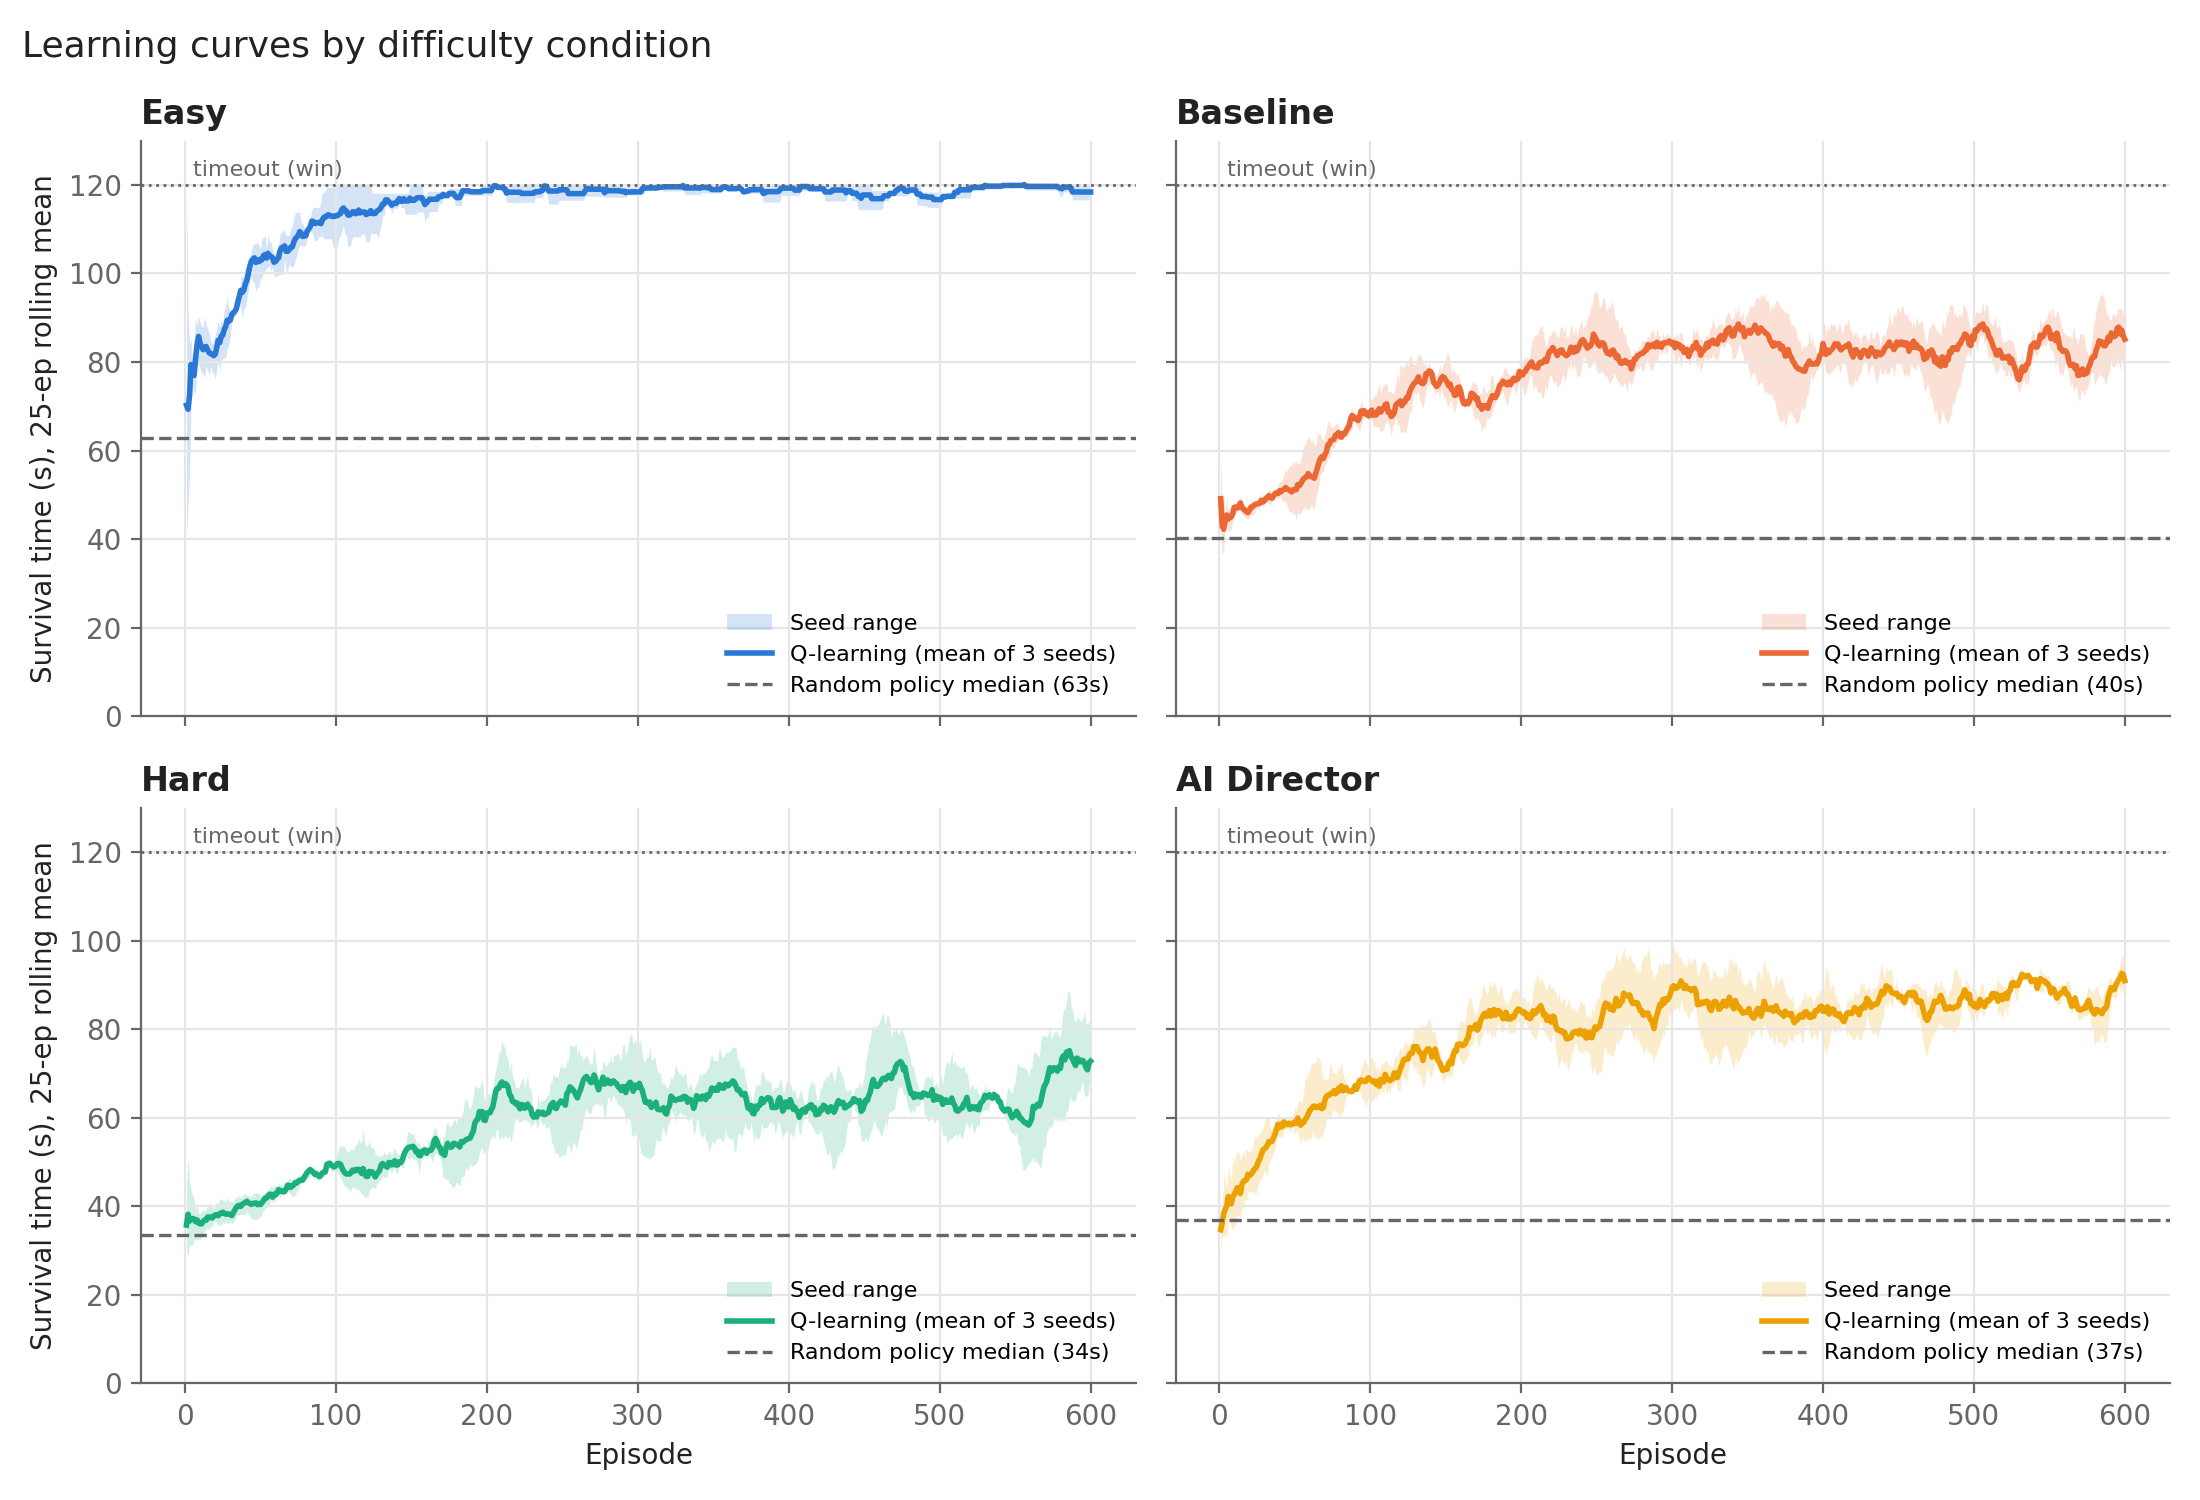
\includegraphics[width=\textwidth]{plots_final/fig1_learning_curves.png}
\caption{Survival time over training (25-episode rolling mean, mean of 3 seeds; shaded =
range across seeds; dashed = random-policy median).}
\label{fig:learning}
\end{figure}
\todo{Describe.}

\begin{figure}[h]
\centering
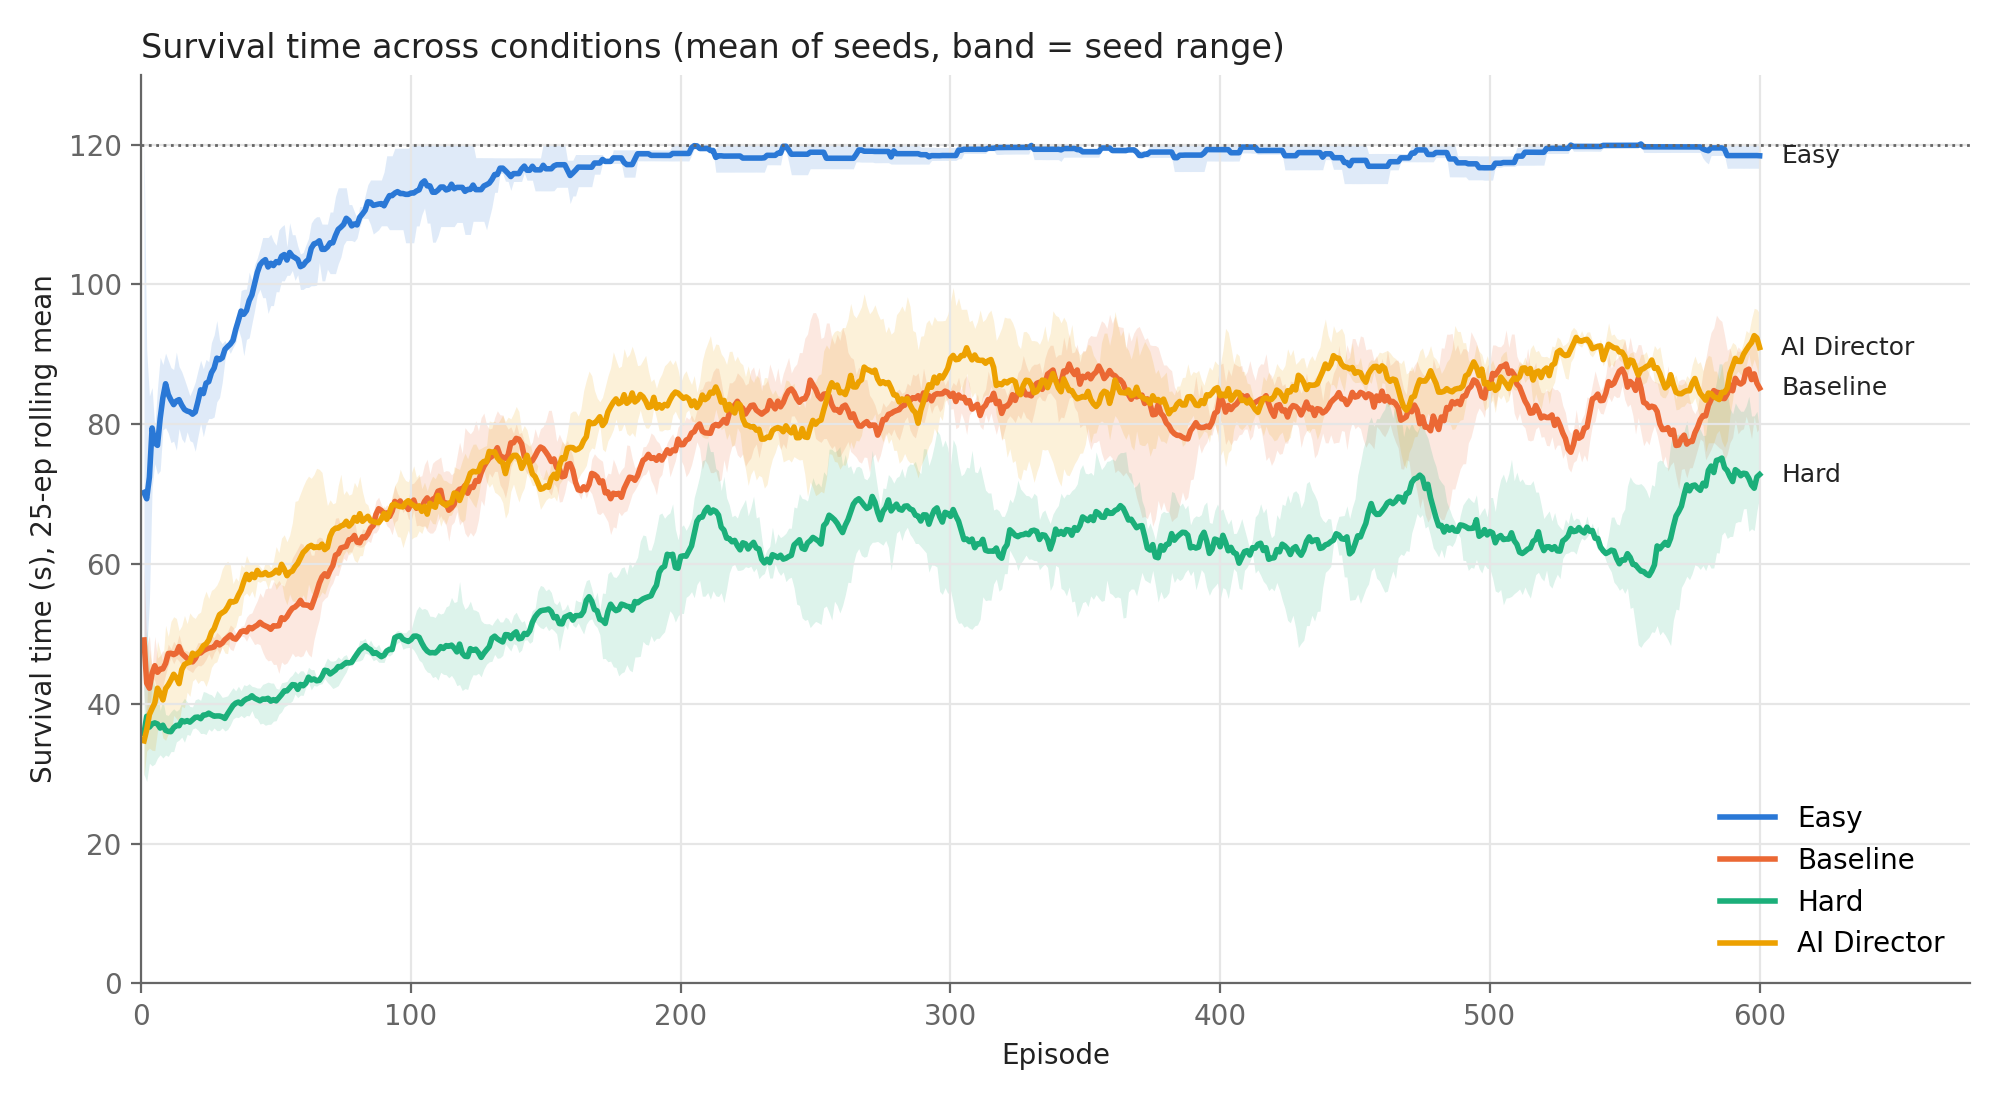
\includegraphics[width=0.85\textwidth]{plots_final/fig2_cross_condition.png}
\caption{Survival time across conditions.}
\label{fig:cross}
\end{figure}

\subsection{Episode return}
\begin{figure}[h]
\centering
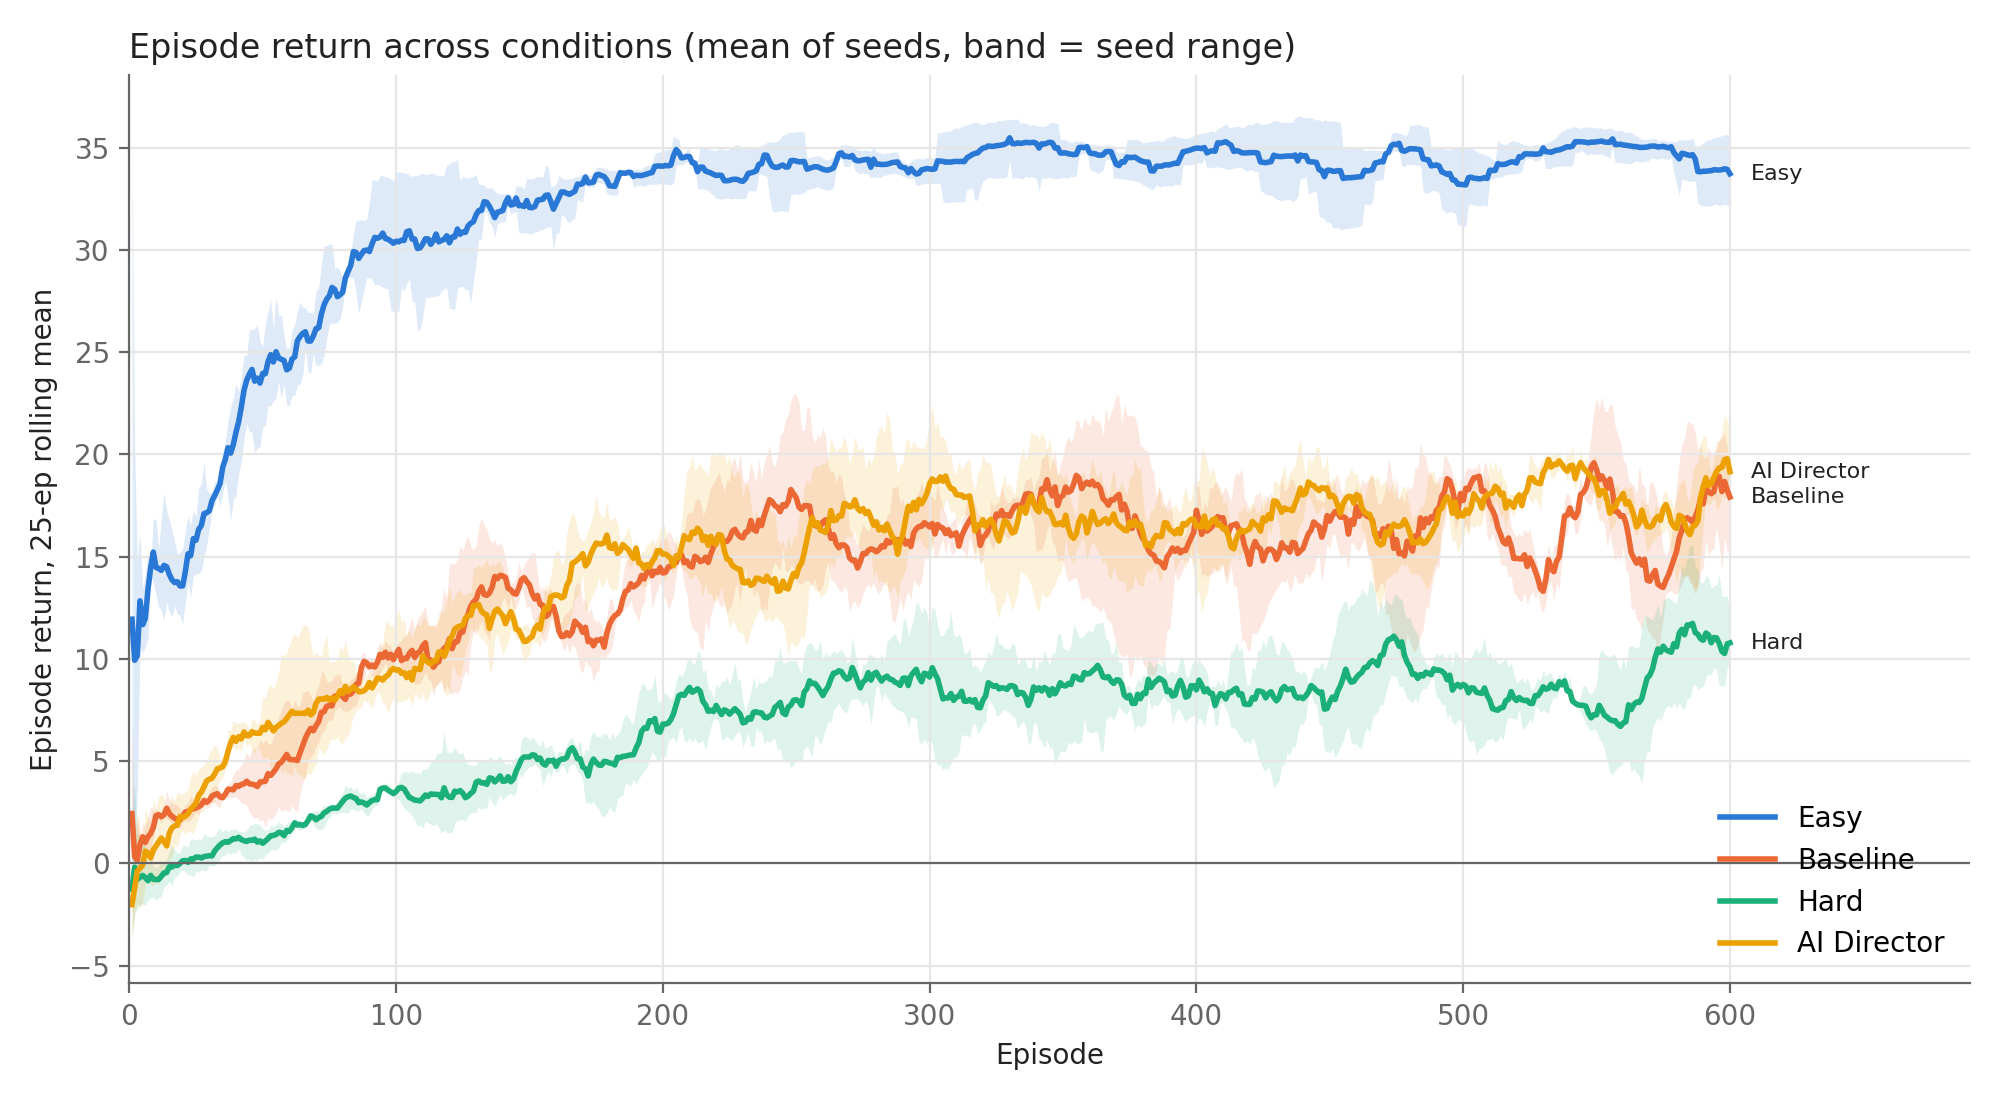
\includegraphics[width=0.85\textwidth]{plots_final/fig6_return_cross_condition.png}
\caption{Episode return across conditions.}
\label{fig:return}
\end{figure}
\todo{Describe.}

\subsection{Win rate}
\begin{figure}[h]
\centering
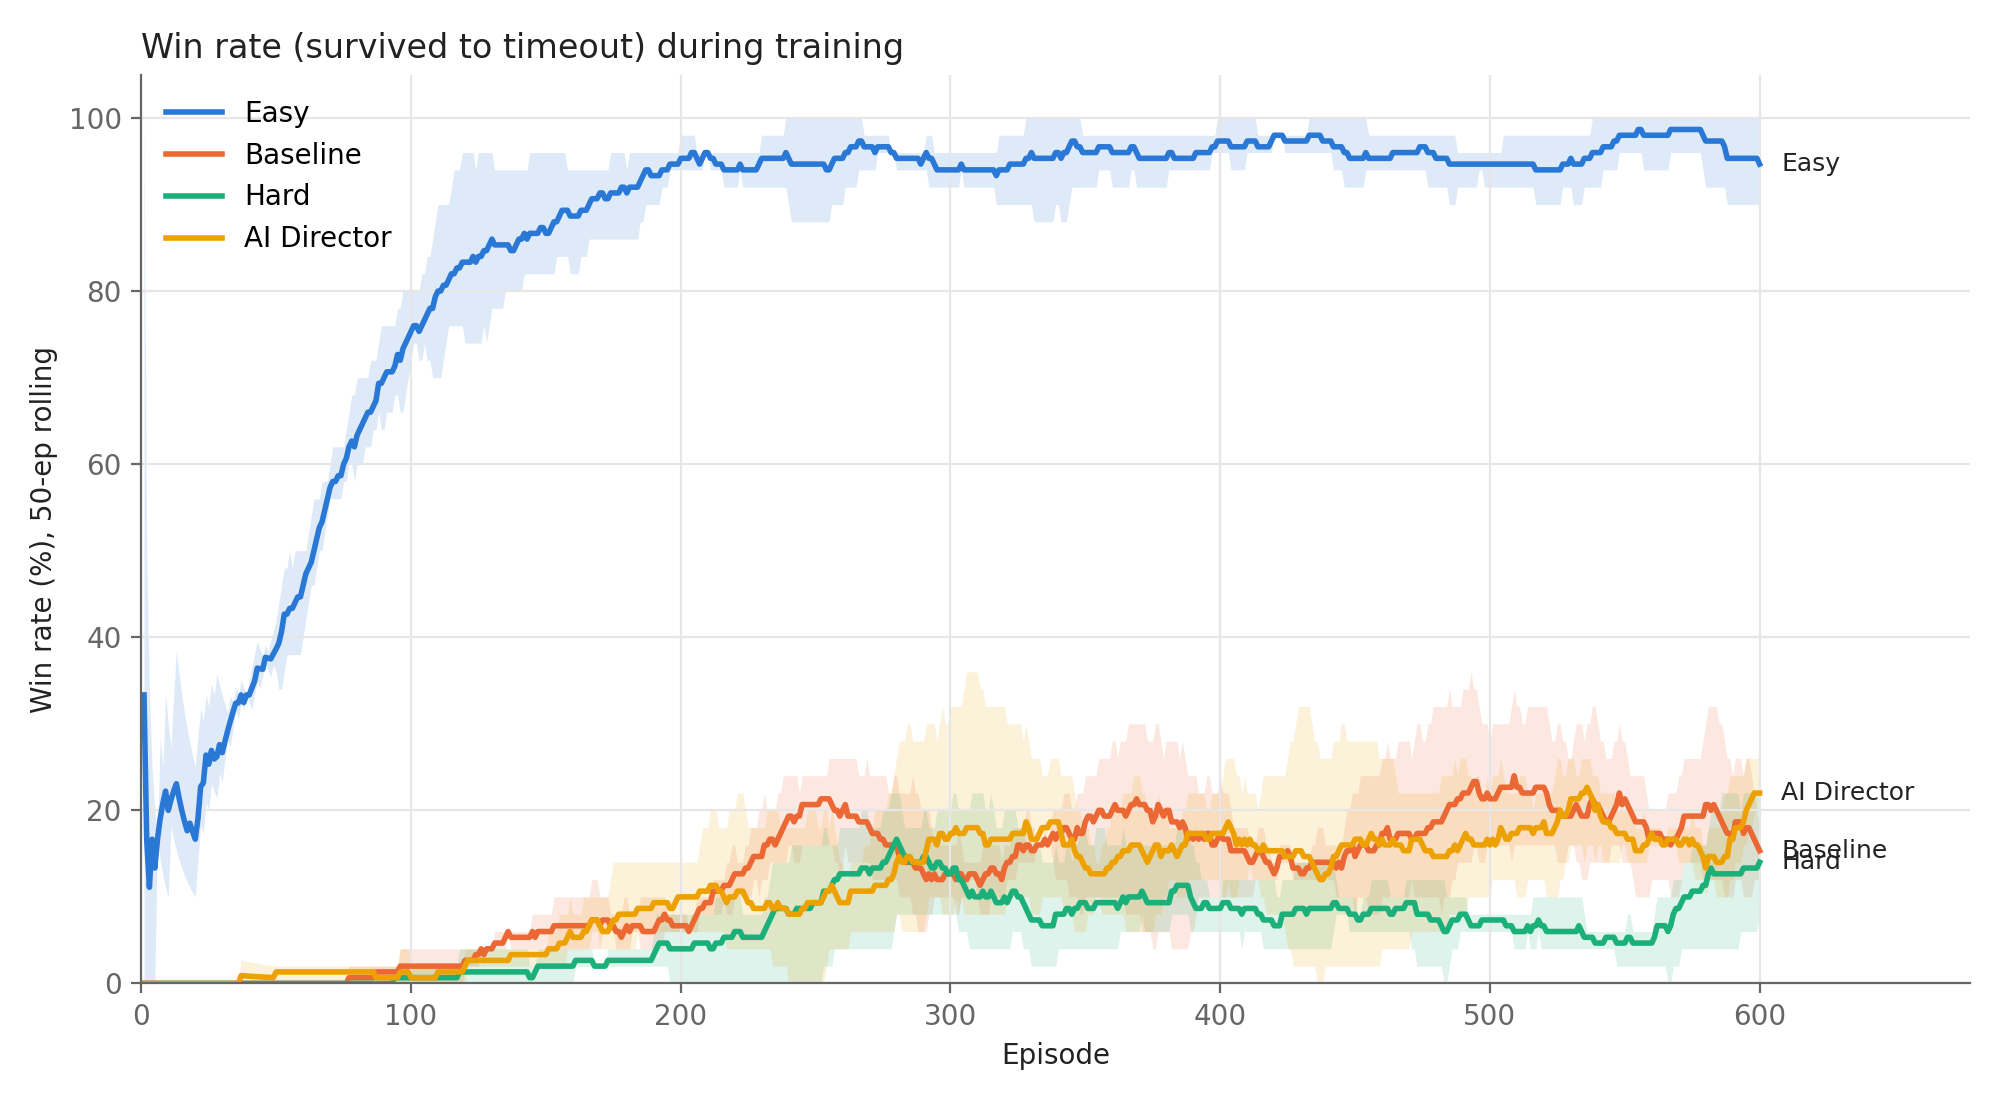
\includegraphics[width=0.85\textwidth]{plots_final/fig3_win_rate.png}
\caption{Rolling win rate (50 episodes) during training.}
\label{fig:win}
\end{figure}

\subsection{Greedy evaluation}
\begin{figure}[h]
\centering
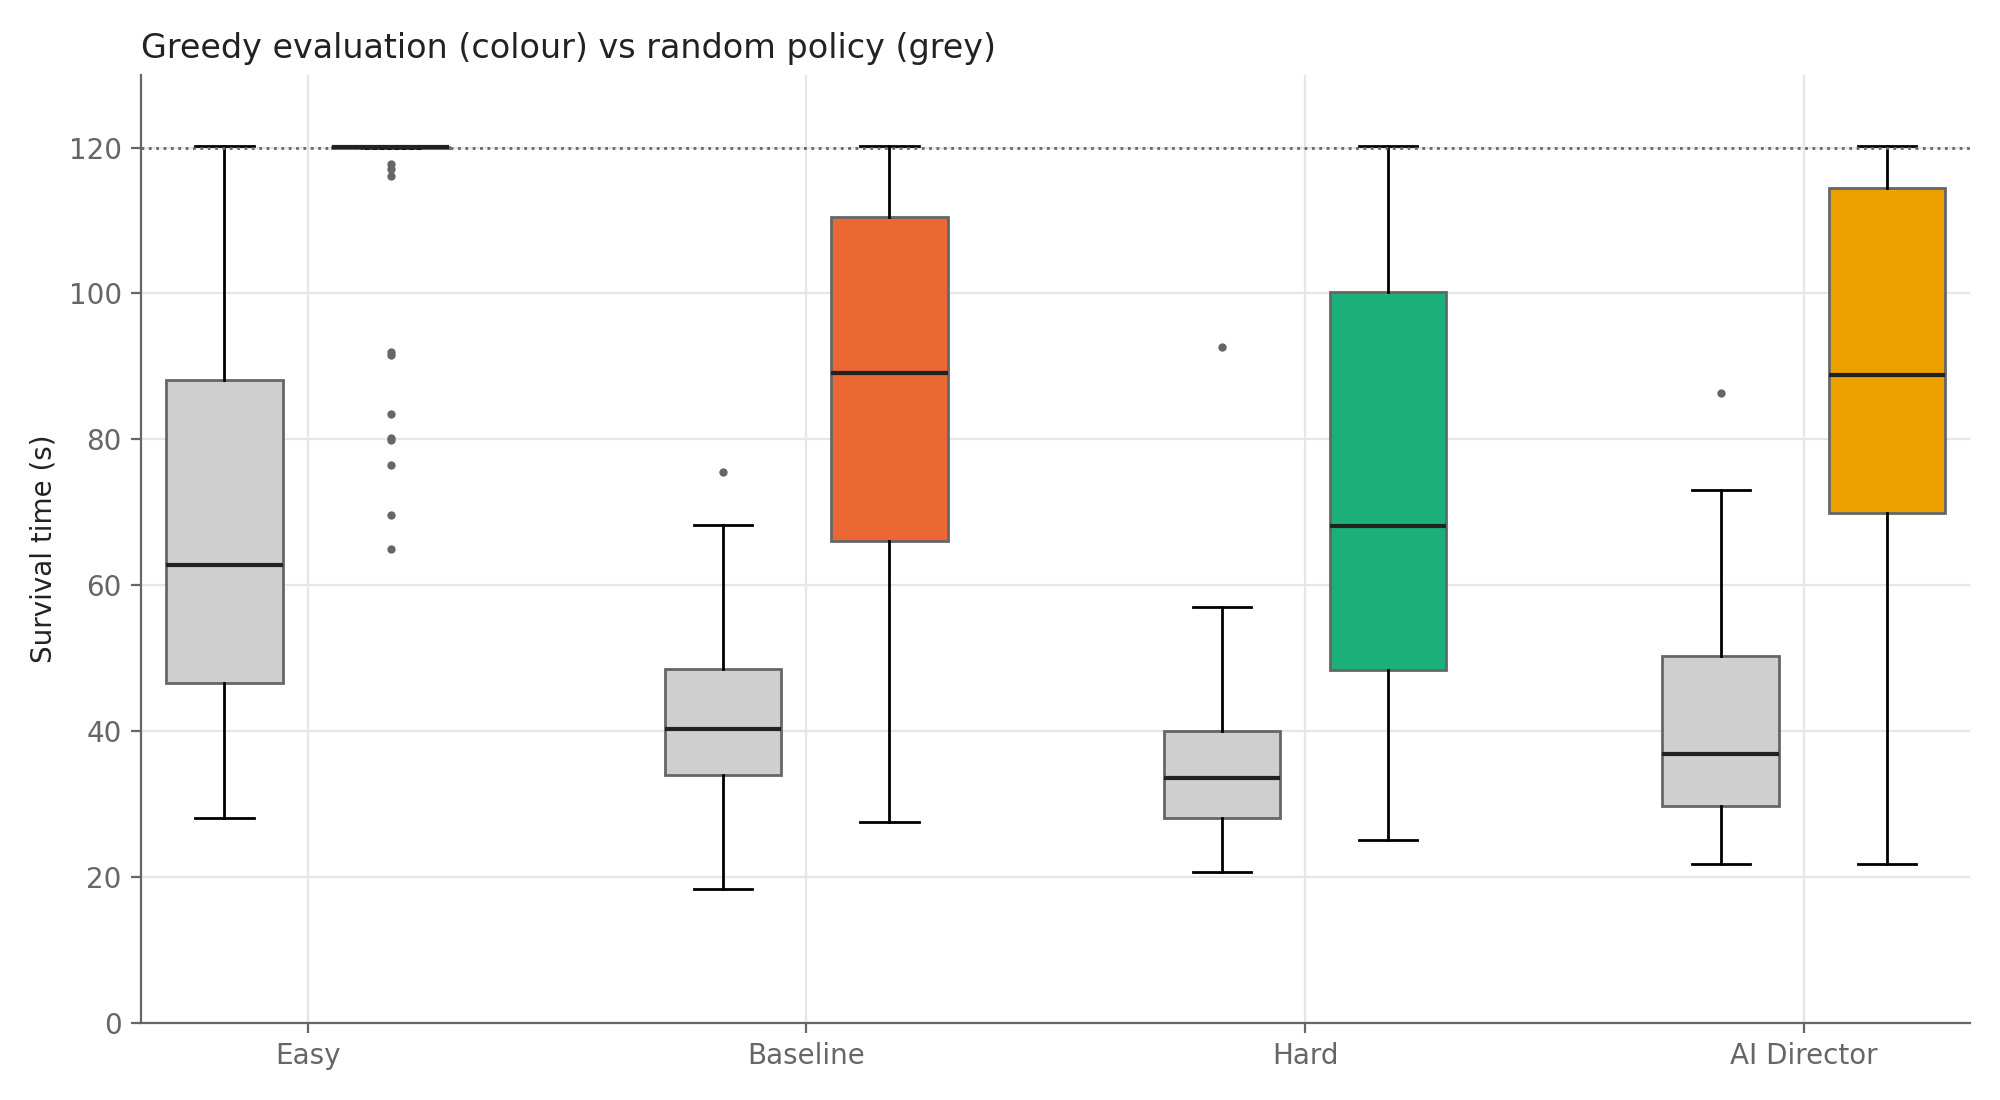
\includegraphics[width=0.85\textwidth]{plots_final/fig4_eval_vs_random.png}
\caption{Survival time of the greedy policy (colour) vs the random policy (grey).}
\label{fig:eval}
\end{figure}

\begin{table}[h]
\centering
\caption{Performance summary (evaluation: 50 episodes $\times$ 3 seeds)}
\label{tab:results}
\begin{tabular}{lcccccc}
\toprule
Condition & \multicolumn{2}{c}{Random} & \multicolumn{3}{c}{Greedy evaluation} & $p$ vs random \\
\cmidrule(lr){2-3}\cmidrule(lr){4-6}
 & Median (s) & Win \% & Median (s) & IQR (s) & Win \% & \\
\midrule
Easy        & 62.8 & 10.0 & 120.1 & 120.0--120.1 & 92.7 & $<10^{-30}$ \\
Baseline    & 40.3 & 0.0  & 89.1  & 66.1--110.5  & 22.0 & $<10^{-30}$ \\
Hard        & 33.6 & 0.0  & 68.2  & 48.4--100.2  & 20.7 & $<10^{-28}$ \\
AI Director & 36.9 & 0.0  & 88.8  & 69.8--114.5  & 18.0 & $<10^{-29}$ \\
\bottomrule
\end{tabular}
\end{table}
\todo{Kruskal--Wallis and pairwise results (see stats\_report.txt).}

\subsection{Behavioural analysis}
\begin{figure}[h]
\centering
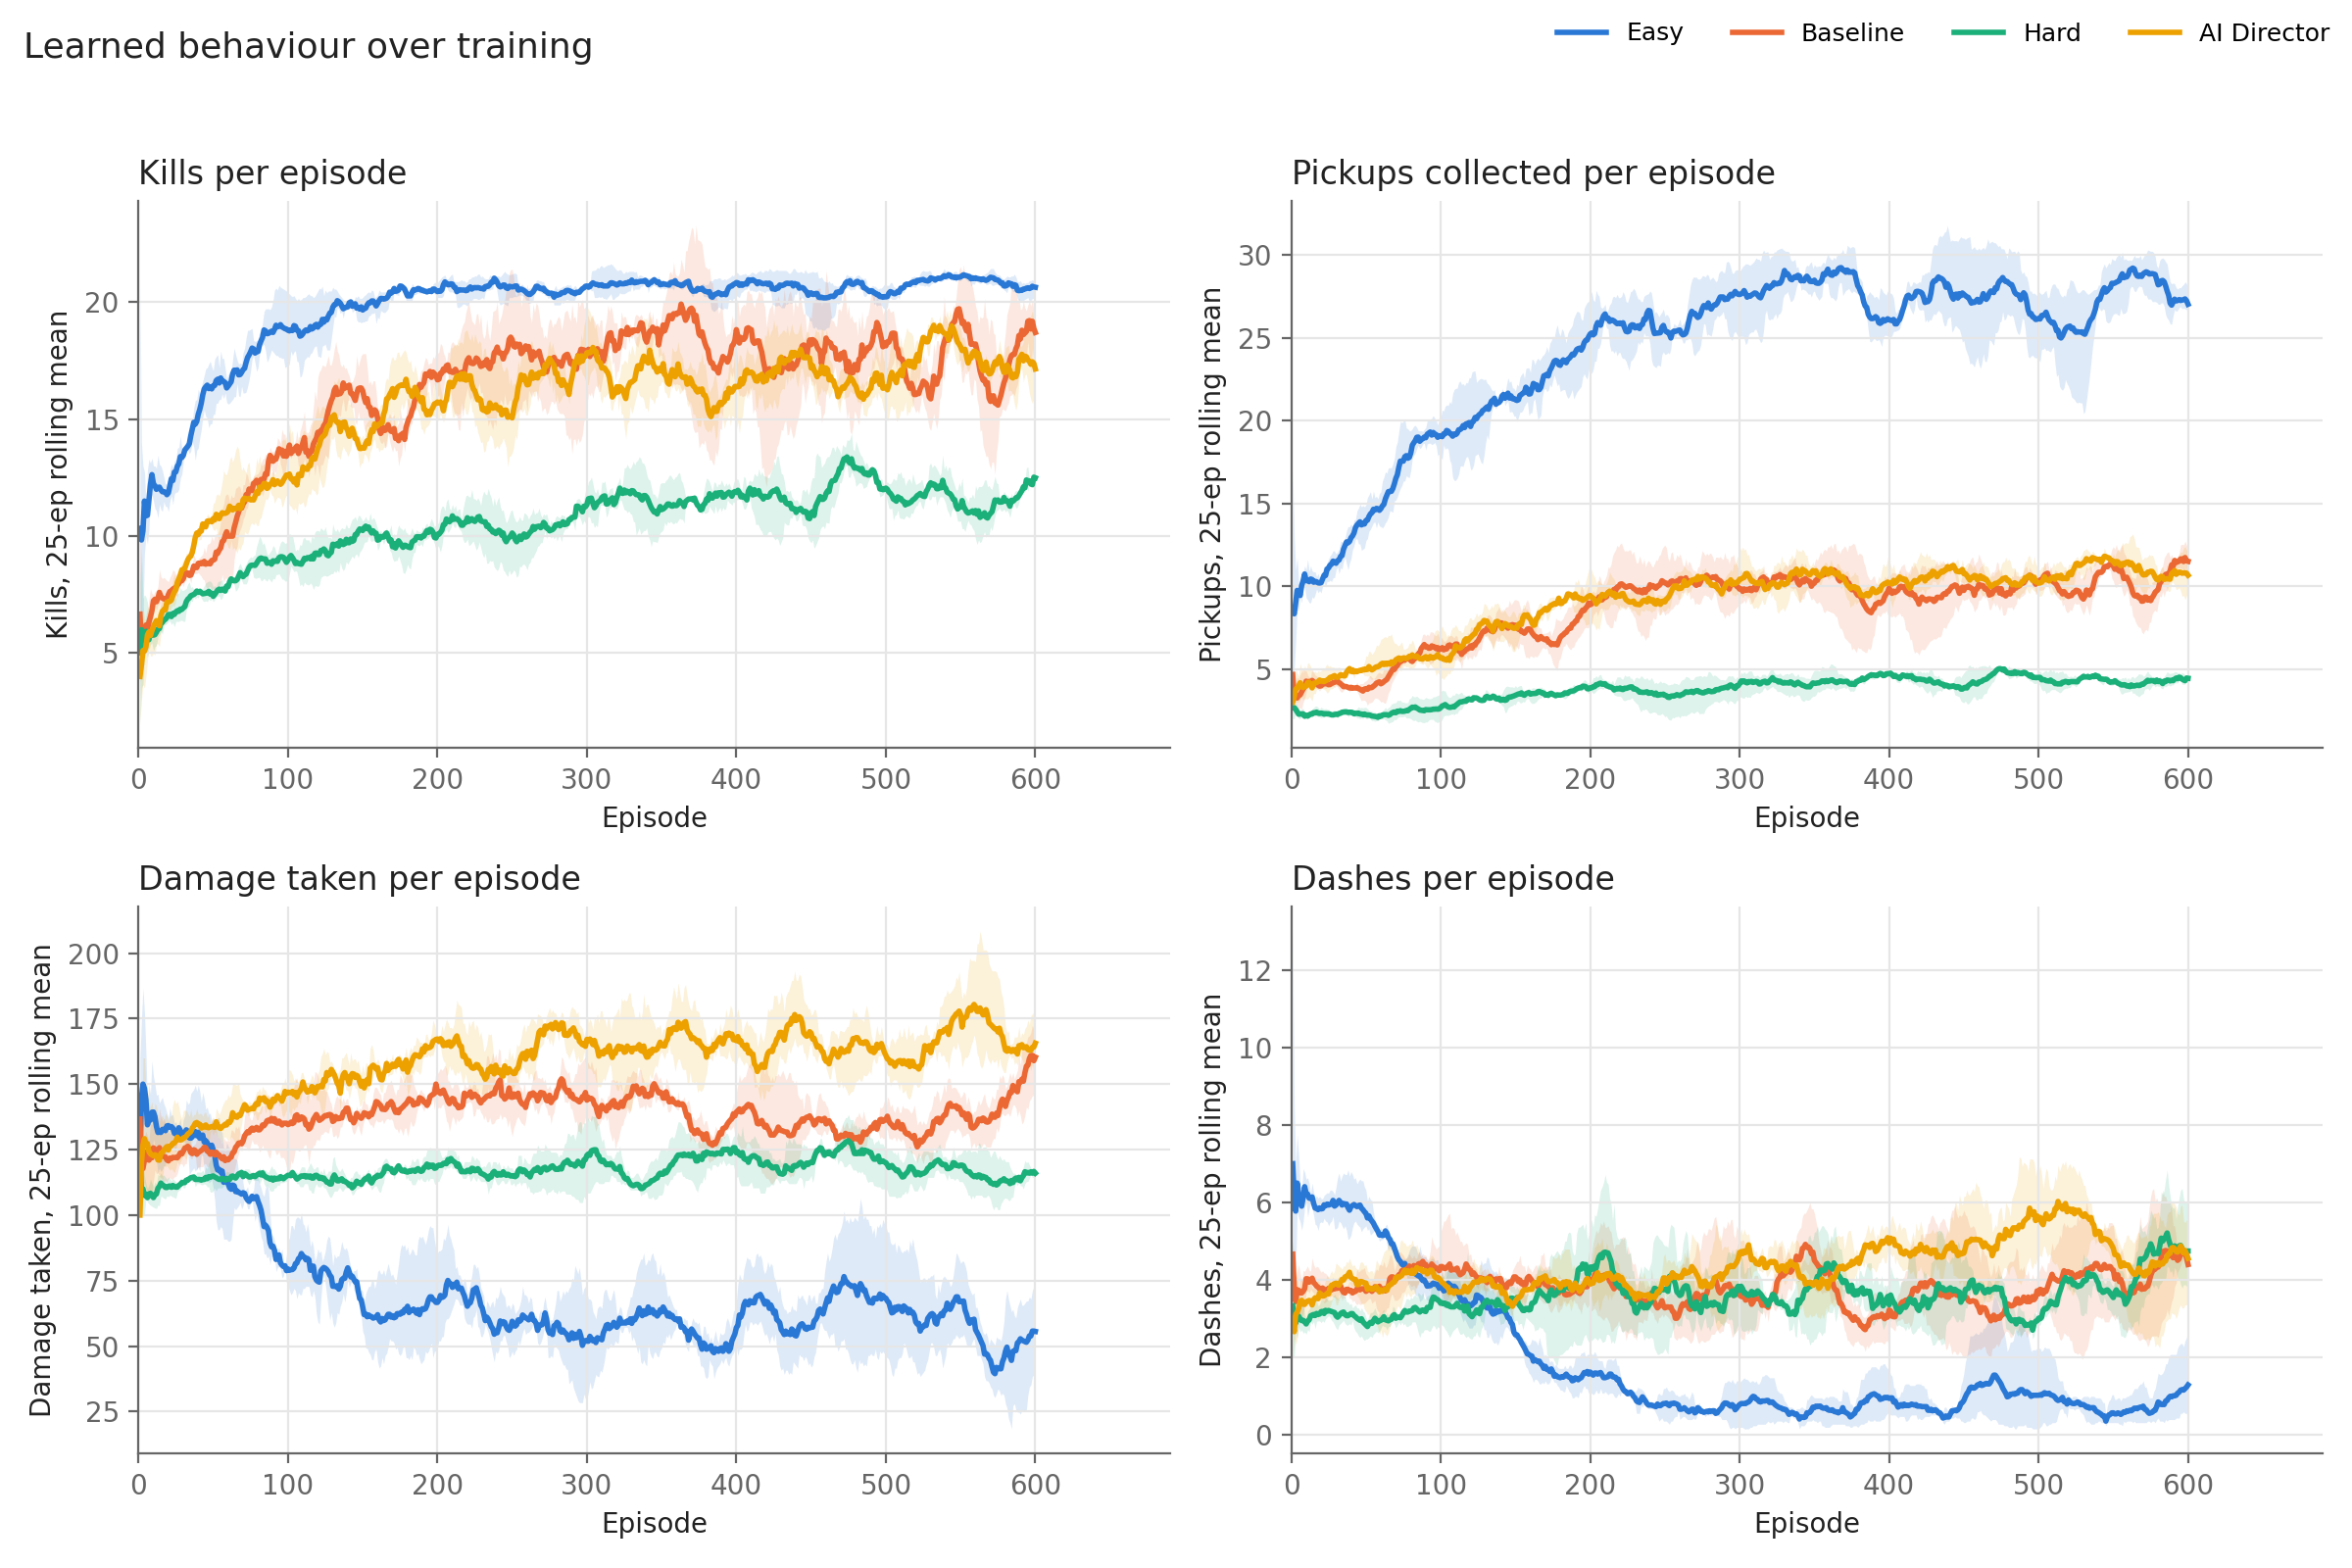
\includegraphics[width=\textwidth]{plots_final/fig7_behaviour.png}
\caption{Kills, pickups, damage taken and dashes per episode over training.}
\label{fig:behaviour}
\end{figure}
\todo{Describe.}

% =====================================================================
\section{Discussion}
\todo{Interpretation, scoped to the evidence.}

\subsection{Limitations}
\todo{Coupled difficulty parameters; AI Director is a package (rests/waves/boss);
Easy ceiling effect; 3 seeds; agent $\neq$ human player; handcrafted tension model.}

\subsection{Future work}
\todo{}

% =====================================================================
\section{Conclusion}
\todo{}

% =====================================================================
\section*{Funding Information}
Authors state no funding involved.

\section*{Author Contributions Statement}
\todo{CRediT table}

\section*{Conflict of Interest Statement}
Authors state no conflict of interest.

\section*{Ethical Approval}
\todo{No human participants were involved; all data were generated in simulation.}

\section*{Data Availability}
\todo{e.g.\ Code and logs are available at ... / from the corresponding author on request.}

% =====================================================================
\begin{thebibliography}{99}
\bibitem{hunicke2005} R.~Hunicke, ``The case for dynamic difficulty adjustment in games,'' in \emph{Proc.\ ACM SIGCHI ACE}, 2005, pp.~429--433.
\bibitem{sutton2018} R.~S.~Sutton and A.~G.~Barto, \emph{Reinforcement Learning: An Introduction}, 2nd~ed. MIT Press, 2018.
\bibitem{singh2000} S.~Singh, T.~Jaakkola, M.~L.~Littman, and C.~Szepesv\'ari, ``Convergence results for single-step on-policy reinforcement-learning algorithms,'' \emph{Machine Learning}, vol.~38, pp.~287--308, 2000.
\bibitem{watkins1992} C.~J.~C.~H.~Watkins and P.~Dayan, ``Q-learning,'' \emph{Machine Learning}, vol.~8, pp.~279--292, 1992.
\bibitem{todo} \todo{carry over remaining references from the previous draft (remove the duplicate Sekhavat entry)}
\end{thebibliography}

\end{document}
